\documentclass{standalone}
\usepackage{tikz}
\usetikzlibrary{patterns, positioning}


\begin{document}
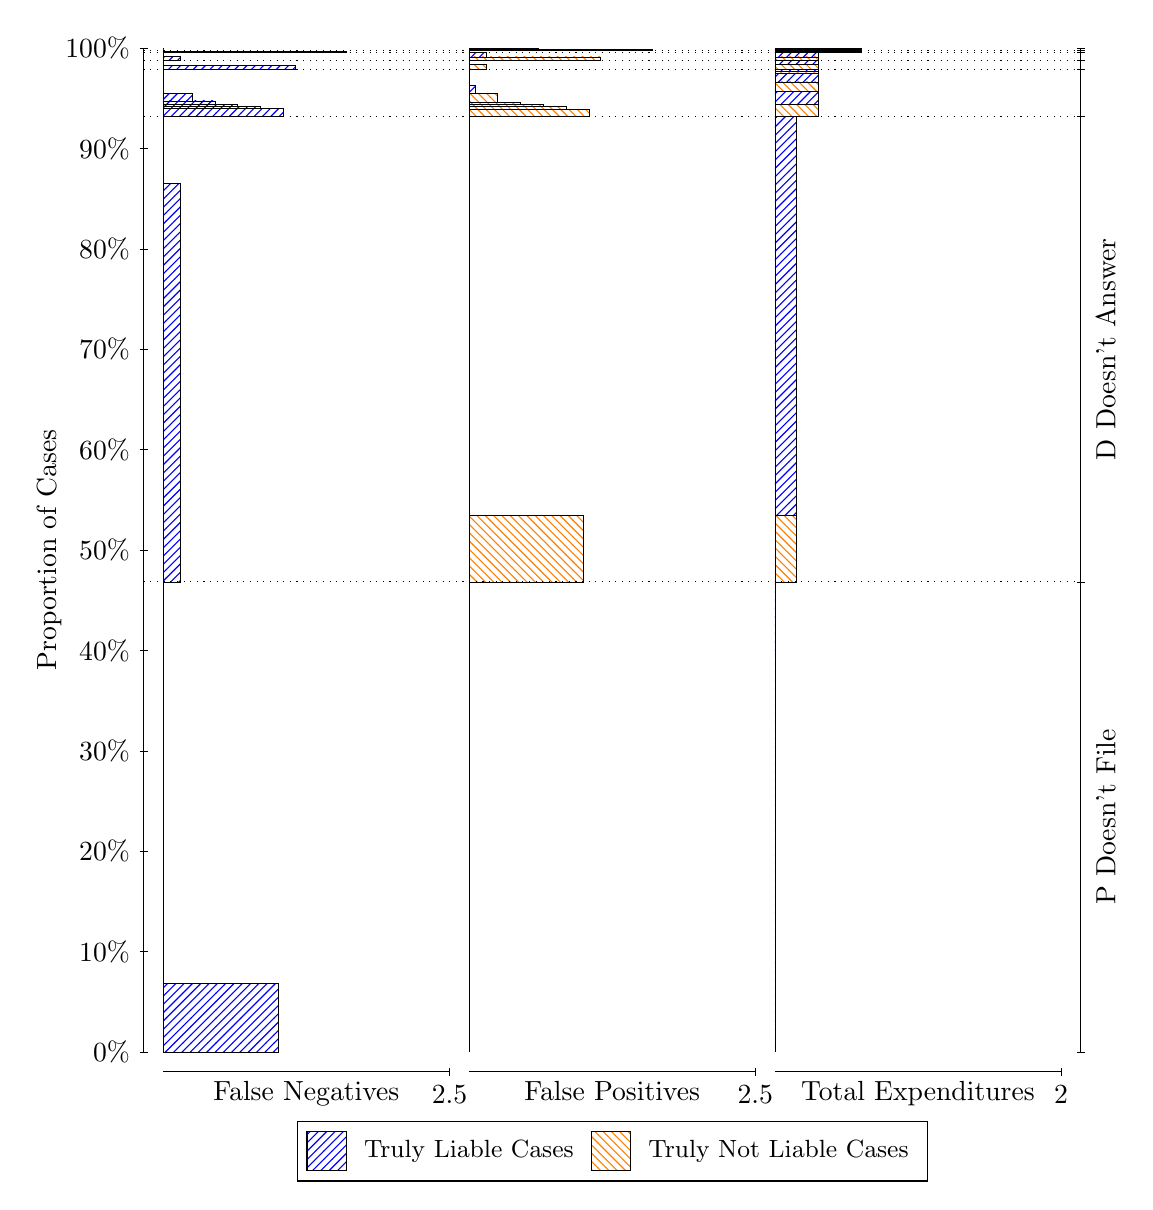
\begin{tikzpicture}
\draw[black, very thin] (1.5,1.75) -- (1.5,14.5);
\node[rotate=90, text=black, anchor=center] at (0.3, 8.125) {Proportion of Cases};
\draw[black, very thin] (1.45,1.75) -- (1.55,1.75);
\node[text=black, anchor=east] at (1.45, 1.75) {0\%};
\draw[black, very thin] (1.45,3.025) -- (1.55,3.025);
\node[text=black, anchor=east] at (1.45, 3.025) {10\%};
\draw[black, very thin] (1.45,4.3) -- (1.55,4.3);
\node[text=black, anchor=east] at (1.45, 4.3) {20\%};
\draw[black, very thin] (1.45,5.575) -- (1.55,5.575);
\node[text=black, anchor=east] at (1.45, 5.575) {30\%};
\draw[black, very thin] (1.45,6.85) -- (1.55,6.85);
\node[text=black, anchor=east] at (1.45, 6.85) {40\%};
\draw[black, very thin] (1.45,8.125) -- (1.55,8.125);
\node[text=black, anchor=east] at (1.45, 8.125) {50\%};
\draw[black, very thin] (1.45,9.4) -- (1.55,9.4);
\node[text=black, anchor=east] at (1.45, 9.4) {60\%};
\draw[black, very thin] (1.45,10.675) -- (1.55,10.675);
\node[text=black, anchor=east] at (1.45, 10.675) {70\%};
\draw[black, very thin] (1.45,11.95) -- (1.55,11.95);
\node[text=black, anchor=east] at (1.45, 11.95) {80\%};
\draw[black, very thin] (1.45,13.225) -- (1.55,13.225);
\node[text=black, anchor=east] at (1.45, 13.225) {90\%};
\draw[black, very thin] (1.45,14.5) -- (1.55,14.5);
\node[text=black, anchor=east] at (1.45, 14.5) {100\%};

\draw[black, very thin] (13.4,1.75) -- (13.4,14.5);
\draw[black, very thin] (13.35,1.75) -- (13.45,1.75);
\node[anchor=west] at (13.35, 1.75) {};
\draw[black, very thin] (13.35,7.7206) -- (13.45,7.7206);
\node[anchor=west] at (13.35, 7.7206) {};
\draw[black, very thin] (13.35,13.628) -- (13.45,13.628);
\node[anchor=west] at (13.35, 13.628) {};
\draw[black, very thin] (13.35,14.228) -- (13.45,14.228);
\node[anchor=west] at (13.35, 14.228) {};
\draw[black, very thin] (13.35,14.339) -- (13.45,14.339);
\node[anchor=west] at (13.35, 14.339) {};
\draw[black, very thin] (13.35,14.447) -- (13.45,14.447);
\node[anchor=west] at (13.35, 14.447) {};
\draw[black, very thin] (13.35,14.473) -- (13.45,14.473);
\node[anchor=west] at (13.35, 14.473) {};
\draw[black, very thin] (13.35,14.5) -- (13.45,14.5);
\node[anchor=west] at (13.35, 14.5) {};

\draw[black, very thin, pattern color=blue, pattern=north east lines] (1.75,1.75) rectangle (3.2033,2.6257);
\draw[black, very thin, pattern color=orange, pattern=north west lines] (1.75,2.6257) rectangle (1.75,7.7206);
\draw[black, very thin, pattern color=blue, pattern=north east lines] (1.75,7.7206) rectangle (1.968,12.784);
\draw[black, very thin, pattern color=orange, pattern=north west lines] (1.75,12.784) rectangle (1.75,13.628);
\draw[black, very thin, pattern color=blue, pattern=north east lines] (1.75,13.628) rectangle (3.276,13.738);
\draw[black, very thin, pattern color=blue, pattern=north east lines] (1.75,13.738) rectangle (2.9853,13.762);
\draw[black, very thin, pattern color=blue, pattern=north east lines] (1.75,13.762) rectangle (2.6947,13.788);
\draw[black, very thin, pattern color=blue, pattern=north east lines] (1.75,13.788) rectangle (2.404,13.828);
\draw[black, very thin, pattern color=blue, pattern=north east lines] (1.75,13.828) rectangle (2.1133,13.928);
\draw[black, very thin, pattern color=orange, pattern=north west lines] (1.75,13.928) rectangle (1.75,14.228);
\draw[black, very thin, pattern color=blue, pattern=north east lines] (1.75,14.228) rectangle (3.4213,14.278);
\draw[black, very thin, pattern color=orange, pattern=north west lines] (1.75,14.278) rectangle (1.75,14.339);
\draw[black, very thin, pattern color=blue, pattern=north east lines] (1.75,14.339) rectangle (1.968,14.398);
\draw[black, very thin, pattern color=orange, pattern=north west lines] (1.75,14.398) rectangle (1.75,14.447);
\draw[black, very thin, pattern color=blue, pattern=north east lines] (1.75,14.447) rectangle (4.0753,14.455);
\draw[black, very thin, pattern color=orange, pattern=north west lines] (1.75,14.455) rectangle (1.75,14.473);
\draw[black, very thin, pattern color=orange, pattern=north west lines] (1.75,14.473) rectangle (1.75,14.482);
\draw[black, very thin, pattern color=blue, pattern=north east lines] (1.75,14.482) rectangle (1.75,14.5);
\draw[black, very thin, pattern color=orange, pattern=north west lines] (5.6333,1.75) rectangle (5.6333,6.8449);
\draw[black, very thin, pattern color=blue, pattern=north east lines] (5.6333,6.8449) rectangle (5.6333,7.7206);
\draw[black, very thin, pattern color=orange, pattern=north west lines] (5.6333,7.7206) rectangle (7.0867,8.5645);
\draw[black, very thin, pattern color=blue, pattern=north east lines] (5.6333,8.5645) rectangle (5.6333,13.628);
\draw[black, very thin, pattern color=orange, pattern=north west lines] (5.6333,13.628) rectangle (7.1593,13.723);
\draw[black, very thin, pattern color=orange, pattern=north west lines] (5.6333,13.723) rectangle (6.8687,13.762);
\draw[black, very thin, pattern color=orange, pattern=north west lines] (5.6333,13.762) rectangle (6.578,13.788);
\draw[black, very thin, pattern color=orange, pattern=north west lines] (5.6333,13.788) rectangle (6.2873,13.813);
\draw[black, very thin, pattern color=orange, pattern=north west lines] (5.6333,13.813) rectangle (5.9967,13.928);
\draw[black, very thin, pattern color=blue, pattern=north east lines] (5.6333,13.928) rectangle (5.706,14.028);
\draw[black, very thin, pattern color=blue, pattern=north east lines] (5.6333,14.028) rectangle (5.6333,14.228);
\draw[black, very thin, pattern color=orange, pattern=north west lines] (5.6333,14.228) rectangle (5.8513,14.289);
\draw[black, very thin, pattern color=blue, pattern=north east lines] (5.6333,14.289) rectangle (5.6333,14.339);
\draw[black, very thin, pattern color=orange, pattern=north west lines] (5.6333,14.339) rectangle (7.3047,14.388);
\draw[black, very thin, pattern color=blue, pattern=north east lines] (5.6333,14.388) rectangle (5.8513,14.447);
\draw[black, very thin, pattern color=orange, pattern=north west lines] (5.6333,14.447) rectangle (5.6333,14.465);
\draw[black, very thin, pattern color=blue, pattern=north east lines] (5.6333,14.465) rectangle (5.6333,14.473);
\draw[black, very thin, pattern color=orange, pattern=north west lines] (5.6333,14.473) rectangle (7.9587,14.482);
\draw[black, very thin, pattern color=blue, pattern=north east lines] (5.6333,14.482) rectangle (6.5053,14.5);
\draw[black, very thin, pattern color=orange, pattern=north west lines] (9.5167,1.75) rectangle (9.5167,6.8449);
\draw[black, very thin, pattern color=blue, pattern=north east lines] (9.5167,6.8449) rectangle (9.5167,7.7206);
\draw[black, very thin, pattern color=orange, pattern=north west lines] (9.5167,7.7206) rectangle (9.7892,8.5645);
\draw[black, very thin, pattern color=blue, pattern=north east lines] (9.5167,8.5645) rectangle (9.7892,13.628);
\draw[black, very thin, pattern color=orange, pattern=north west lines] (9.5167,13.628) rectangle (10.062,13.788);
\draw[black, very thin, pattern color=blue, pattern=north east lines] (9.5167,13.788) rectangle (10.062,13.954);
\draw[black, very thin, pattern color=orange, pattern=north west lines] (9.5167,13.954) rectangle (10.062,14.069);
\draw[black, very thin, pattern color=blue, pattern=north east lines] (9.5167,14.069) rectangle (10.062,14.179);
\draw[black, very thin, pattern color=orange, pattern=north west lines] (9.5167,14.179) rectangle (10.062,14.203);
\draw[black, very thin, pattern color=blue, pattern=north east lines] (9.5167,14.203) rectangle (10.062,14.228);
\draw[black, very thin, pattern color=orange, pattern=north west lines] (9.5167,14.228) rectangle (10.062,14.289);
\draw[black, very thin, pattern color=blue, pattern=north east lines] (9.5167,14.289) rectangle (10.062,14.339);
\draw[black, very thin, pattern color=orange, pattern=north west lines] (9.5167,14.339) rectangle (10.062,14.388);
\draw[black, very thin, pattern color=blue, pattern=north east lines] (9.5167,14.388) rectangle (10.062,14.447);
\draw[black, very thin, pattern color=orange, pattern=north west lines] (9.5167,14.447) rectangle (10.607,14.465);
\draw[black, very thin, pattern color=blue, pattern=north east lines] (9.5167,14.465) rectangle (10.607,14.473);
\draw[black, very thin, pattern color=orange, pattern=north west lines] (9.5167,14.473) rectangle (10.607,14.482);
\draw[black, very thin, pattern color=blue, pattern=north east lines] (9.5167,14.482) rectangle (10.607,14.5);
\draw[black, dotted] (1.5,7.7206) -- (13.4,7.7206);
\draw[black, dotted] (1.5,13.628) -- (13.4,13.628);
\draw[black, dotted] (1.5,14.228) -- (13.4,14.228);
\draw[black, dotted] (1.5,14.339) -- (13.4,14.339);
\draw[black, dotted] (1.5,14.447) -- (13.4,14.447);
\draw[black, dotted] (1.5,14.473) -- (13.4,14.473);
\draw[black, very thin] (1.75,1.5) -- (5.3833,1.5);
\node[text=black, anchor=north] at (3.5667, 1.5) {False Negatives};
\draw[black, very thin] (5.3833,1.45) -- (5.3833,1.55);
\node[text=black, anchor=north] at (5.3833, 1.45) {2.5};

\draw[black, very thin] (5.6333,1.5) -- (9.2667,1.5);
\node[text=black, anchor=north] at (7.45, 1.5) {False Positives};
\draw[black, very thin] (9.2667,1.45) -- (9.2667,1.55);
\node[text=black, anchor=north] at (9.2667, 1.45) {2.5};

\draw[black, very thin] (9.5167,1.5) -- (13.15,1.5);
\node[text=black, anchor=north] at (11.333, 1.5) {Total Expenditures};
\draw[black, very thin] (13.15,1.45) -- (13.15,1.55);
\node[text=black, anchor=north] at (13.15, 1.45) {2};

\node[text=black, centered, rotate=90] at (13.72, 4.7353) {P Doesn't File};
\node[text=black, centered, rotate=90] at (13.72, 10.674) {D Doesn't Answer};






\draw (7.449999999999999,1.5) node[draw=none] (baseCoordinate) {};
\begin{scope}[align=center]
        \matrix[scale=0.5, draw=black, below=0.5cm of baseCoordinate, nodes={draw}, column sep=0.1cm]{
            \node[rectangle, draw, minimum width=0.5cm, minimum height=0.5cm, pattern color=blue, pattern=north east lines] {}; &
            \node[draw=none, font=\small, text=black] (B) {Truly Liable Cases}; &
            \node[rectangle, draw, minimum width=0.5cm, minimum height=0.5cm, pattern color=orange, pattern=north west lines] {}; &
            \node[draw=none, font=\small, text=black] (B) {Truly Not Liable Cases}; \\
            };
\end{scope}

\end{tikzpicture}
\end{document}